\newpage
\begin{figure}[h]
	\centering
	\caption{UCA 4 - Inserimento modalità di tracciamento}
	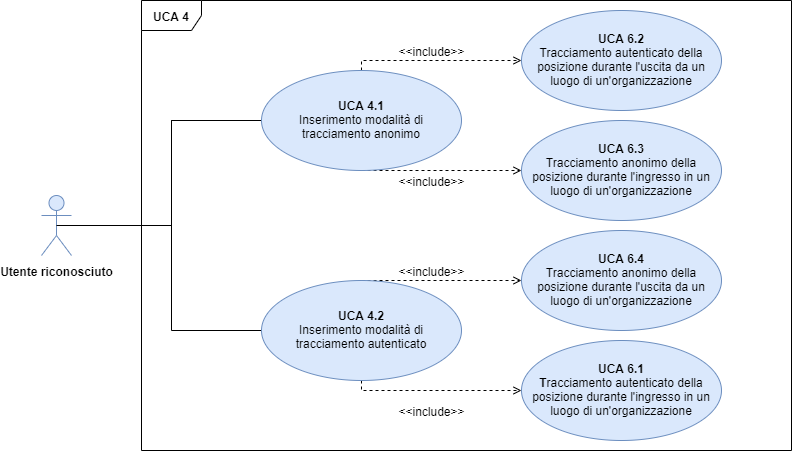
\includegraphics[scale=0.53]{sezioni/UseCase/Immagini/UCA4.png}
\end{figure}
\section{UCA 4 - Inserimento modalità di tracciamento}%kite level
\begin{itemize}
	\item \textbf{Attori primari:} Utente riconosciuto;
	\item \textbf{Precondizione:} L'utente si è autenticato con le credenziali LDAP\ap{G} nella organizzazione in cui si trova e vuole selezionare la modalita di tracciamento;
	\item \textbf{Postcondizione:} L'utente viene tracciato secondo la modalità scelta da lui precedentemente; 
	\item \textbf{Scenario principale:} L'utente accede alla funzionali di "Inserimento modalità di tracciamento" scegliendo tra:
	\begin{itemize}
		\item UCA 6.1 Inserimento modalità anonimo\ap{G};
		\item UCA 6.2 Inserimento modalità autenticato\ap{G}.
	\end{itemize}
\end{itemize}

\subsection{UCA 4.1 - Inserimento modalità anonimo}%sea level
\begin{itemize}
\item \textbf{Attori primari:} Utente riconosciuto;
\item \textbf{Precondizione:} L'utente si è autenticato con le credenziali LDAP\ap{G} nella organizzazione in cui si trova e vuole selezionare la modalita di tracciamento anonimo
\item \textbf{Postcondizione:}  L'utente viene tracciato secondo la modalità anonimo;
\item \textbf{Scenario principale:}
	\begin{itemize}
	\item L'utente accede alla funzionalita inserimento modalità di tracciamento;
	\item L'utente inserisce la modalità anonimo.
\end{itemize}
\end{itemize}

\subsection{UCA 4.2 - Inserimento modalità autenticato}%sea level
\begin{itemize}
	\item \textbf{Attori primari:} Utente riconosciuto;
	\item \textbf{Precondizione:} L'utente si è autenticato con le credenziali LDAP\ap{G} nella organizzazione in cui si trova e vuole selezionare la modalita di tracciamento autenticato;
	\item \textbf{Postcondizione:}  L'utente viene tracciato secondo la modalità autenticato;
	\item \textbf{Scenario principale:}
	\begin{itemize}
		\item L'utente accede alla funzionalita inserimento modalità di tracciamento;
		\item L'utente inserisce la modalità autenticato.
	\end{itemize}
\end{itemize}
